\begin{table}[t]
\centering
\caption{Macro-F1 for germ-cell stage annotation under six train/test settings (left three in-distribution, right three shifted); mean over test pucks, $\pm$ standard deviation across test pucks. nbr: mean embedding of the 15 nearest spatial neighbours. $\alpha$ was selected on the WT$\to$WT folds. MLP rows are in Table~\ref{tab:germ4full}.}
\label{tab:main}
\footnotesize
\setlength{\tabcolsep}{2.5pt}
\input{../results/table_germ4_main.tex}
\end{table}

\begin{figure}[t]
\centering
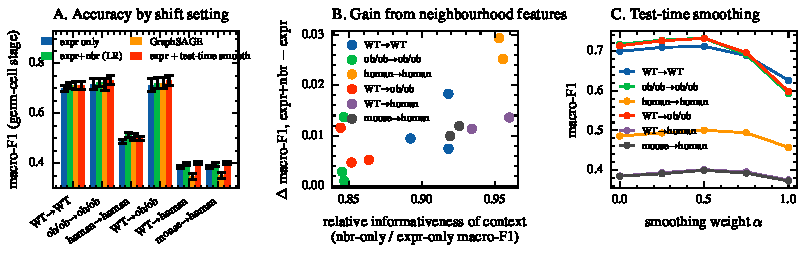
\includegraphics[width=\linewidth]{figs/fig_main.pdf}
\caption{(A) Germ-cell stage macro-F1 by shift setting; error bars are standard deviations across test pucks. (B) Gain from neighbourhood features per test puck against the relative informativeness of context (macro-F1 of a neighbourhood-only classifier divided by that of the expression-only classifier). (C) Test-time smoothing of the expression-only posterior against the weight $\alpha$; $\alpha=1$ replaces each bead's posterior by its neighbours' mean.}
\label{fig:main}
\end{figure}

\paragraph{In-distribution gains are small and consistent.} On held-out WT pucks, the expression-only logistic regression reaches 0.699 macro-F1, and every form of spatial context adds about one point: neighbourhood-augmented LR 0.711, GraphSAGE 0.711, and test-time smoothing 0.712 (Table~\ref{tab:main}, Fig.~\ref{fig:main}A). The neighbourhood alone, without the bead's own expression, reaches 0.636, so most of the stage signal is in the bead itself. Gains are similar on \emph{ob/ob} and larger on human folds, where the expression-only ceiling is lower (0.486) and neighbourhood features add 2.7 points (0.513). Neighbourhood size matters little: $k\in\{5,15,30\}$ changes macro-F1 by at most 0.008 (Table~\ref{tab:sweeps}). An MLP on the same features is 0.6 to 2.1 points below the LR in every setting (Table~\ref{tab:germ4full}).

\paragraph{The \emph{ob/ob} shift is small for this task.} Models trained on WT pucks and applied to \emph{ob/ob} pucks perform as well as models trained on other \emph{ob/ob} pucks (0.713 vs.\ 0.717 for expression only; 0.721 vs.\ 0.723 with neighbourhood features). The spatial gains carry over unchanged, and germ-cell homogeneity overlaps between conditions (0.49 to 0.57 vs.\ 0.53 to 0.56), so at this resolution the disruption reported by \citet{chen2021dissecting} does not register as a distribution shift for stage annotation.

\paragraph{Species shift is large and is dominated by expression.} Expression-only macro-F1 falls from 0.486 (human$\to$human) to 0.385 (WT$\to$human), and adding the \emph{ob/ob} pucks to training does not change it (0.385). Neighbourhood-augmented LR retains a gain under species shift (0.398, $+1.3$), as does test-time smoothing (0.401, $+1.6$). GraphSAGE does not: it is within 0.008 of neighbourhood-augmented LR in every in-distribution setting and becomes the worst model across species, at 0.347 ($-3.8$ vs.\ expression only, $-5.1$ vs.\ neighbourhood LR; seed-to-seed SD $\le 0.007$). Per stage (Fig.~\ref{fig:perclass} in the appendix), the loss is concentrated on round spermatids, the largest human class, whose F1 drops from 0.390 to 0.237 with GraphSAGE and to 0.376 with neighbourhood LR; with neighbourhood LR, spermatogonia and spermatocytes still gain about 3 points.

\paragraph{What predicts the gain.} The gain from context does not track the neighbourhood homogeneity of the target puck: the largest gains occur on the human pucks, which have the lowest homogeneity (0.38 to 0.40). What tracks the gain is instead how informative the neighbourhood is relative to the bead (Fig.~\ref{fig:main}B): the ratio of neighbourhood-only to expression-only macro-F1 is 0.84 to 0.92 for mouse targets, where gains are 0.1 to 1.8 points, and 0.92 to 0.96 for human targets, where gains are 1.0 to 2.9 points. Test-time smoothing peaks at $\alpha=0.5$ in every setting (Fig.~\ref{fig:main}C); replacing the bead's posterior by its neighbours' ($\alpha=1$) costs 7 to 12 points on mouse and 1 to 3 on human targets. At the bead level, the within-species gain is concentrated in the lowest-UMI tertile ($+2.3$ accuracy points on WT$\to$WT, $+4.7$ on human$\to$human, near zero elsewhere), and context lowers accuracy for beads whose neighbourhoods are heterogeneous (Table~\ref{tab:strat}).

